% =====================================================================
%  Factorio Forge --- Whitepaper
%  LLM-Driven Quality-Diversity Search for Emergent Factory Design
%  Engine: pdflatex + bibtex (see Makefile)
% =====================================================================
\documentclass[11pt,a4paper]{article}

% ---------- Encoding & language ----------
\usepackage[T1]{fontenc}
\usepackage[utf8]{inputenc}
\usepackage[english]{babel}
\usepackage{lmodern}
\usepackage{microtype}

% ---------- Layout ----------
\usepackage[a4paper,margin=2.5cm,headheight=22pt]{geometry}
\usepackage{setspace}
\setstretch{1.06}
\usepackage{enumitem}
\setlist{itemsep=2pt,topsep=4pt}

% ---------- Color palette ----------
\usepackage{xcolor}
\definecolor{forgeNavy}{HTML}{1F2A44}   % primary headings
\definecolor{forgeSteel}{HTML}{3D6FB4}  % accent / links
\definecolor{forgeCopper}{HTML}{B05A2A} % warm accent (Factorio-ish)
\definecolor{forgeAsh}{HTML}{6B7280}    % muted gray
\definecolor{notionBlue}{HTML}{2E5E8C}
\definecolor{notionBG}{HTML}{EAF1F8}
\definecolor{toolGreen}{HTML}{2F6B45}
\definecolor{toolBG}{HTML}{E8F3EC}
\definecolor{ruleGray}{HTML}{D8DCE2}

% ---------- Graphics ----------
\usepackage{graphicx}
\usepackage{tikz}
\usetikzlibrary{arrows.meta,positioning,shapes.geometric,fit,backgrounds,calc}
\usepackage{pgfplots}
\pgfplotsset{compat=newest}

% ---------- Tables ----------
\usepackage{booktabs}
\usepackage{tabularx}
\usepackage{array}
\usepackage{multirow}
\newcolumntype{L}[1]{>{\raggedright\arraybackslash}p{#1}}

% ---------- Captions ----------
\usepackage{caption}
\captionsetup{font=small,labelfont={bf,color=forgeNavy},labelsep=period}

% ---------- Pedagogical boxes ----------
\usepackage[most]{tcolorbox}

\newtcolorbox{notionbox}[1]{
  breakable, enhanced,
  colback=notionBG, colframe=notionBlue,
  coltitle=white, fonttitle=\bfseries\sffamily,
  title={Notion --- #1},
  boxrule=0.6pt, left=8pt, right=8pt, top=6pt, bottom=6pt,
  arc=2pt, attach boxed title to top left={xshift=8pt,yshift=-2pt},
  boxed title style={colback=notionBlue,arc=1pt}
}

\newtcolorbox{toolbox}[1]{
  breakable, enhanced,
  colback=toolBG, colframe=toolGreen,
  coltitle=white, fonttitle=\bfseries\sffamily,
  title={Existing project --- #1},
  boxrule=0.6pt, left=8pt, right=8pt, top=6pt, bottom=6pt,
  arc=2pt, attach boxed title to top left={xshift=8pt,yshift=-2pt},
  boxed title style={colback=toolGreen,arc=1pt}
}

% ---------- Section styling ----------
\usepackage{titlesec}
\titleformat{\section}{\Large\bfseries\sffamily\color{forgeNavy}}{\thesection}{0.6em}{}
\titleformat{\subsection}{\large\bfseries\sffamily\color{forgeSteel}}{\thesubsection}{0.6em}{}
\titleformat{\subsubsection}{\normalsize\bfseries\sffamily\color{forgeAsh}}{\thesubsubsection}{0.6em}{}
\titlespacing*{\section}{0pt}{16pt}{8pt}

% ---------- Header / footer ----------
\usepackage{fancyhdr}
\pagestyle{fancy}
\fancyhf{}
\renewcommand{\headrulewidth}{0.6pt}
\renewcommand{\headrule}{\hbox to\headwidth{\color{forgeSteel}\leaders\hrule height \headrulewidth\hfill}}
\fancyhead[L]{\small\sffamily\color{forgeAsh}Factorio Forge}
\fancyhead[R]{\small\sffamily\color{forgeAsh}Whitepaper}
\fancyfoot[C]{\small\sffamily\color{forgeAsh}\thepage}

% ---------- Typography niceties ----------
\widowpenalty=10000
\clubpenalty=10000
\setlength{\parindent}{0pt}
\setlength{\parskip}{0.55em}

% ---------- Cross-references & hyperlinks ----------
\usepackage[colorlinks=true,
            linkcolor=forgeSteel,
            citecolor=forgeCopper,
            urlcolor=forgeSteel]{hyperref}
\usepackage{cleveref}
\hypersetup{
  pdftitle={Factorio Forge: LLM-Driven Quality-Diversity Search for Emergent Factory Design},
  pdfauthor={Geraud (with Claude Code)},
  pdfsubject={Automated optimization, Quality-Diversity, Factorio},
  pdfkeywords={Factorio, MAP-Elites, Quality-Diversity, AlphaEvolve, autoresearch, speedrun}
}

% =====================================================================
\begin{document}

% ------------------------- Title page --------------------------------
\begin{titlepage}
\centering
\vspace*{1.5cm}

{\sffamily\color{forgeAsh}\large A research whitepaper}\\[0.4cm]
{\color{ruleGray}\rule{0.6\textwidth}{0.8pt}}\\[1.0cm]

{\sffamily\bfseries\color{forgeNavy}\Huge Factorio Forge\par}
\vspace{0.7cm}
{\sffamily\large\color{forgeSteel} LLM-Driven Quality-Diversity Search\\[0.2cm] for Emergent Factory Design\par}
\vspace{0.5cm}
{\itshape\color{forgeAsh}\large Can an automated optimization loop discover\\ production structures that humans would not?\par}

\vspace{1.4cm}
{\color{ruleGray}\rule{0.6\textwidth}{0.8pt}}\\[1.0cm]

{\large\sffamily\textbf{G\'eraud}\\[0.2cm]
\color{forgeAsh}with Claude Code\par}

\vfill

% Small TikZ motif: an archive of cells, a few illuminated.

\begin{tikzpicture}[scale=0.5]
  \foreach \x in {0,...,9}{
    \foreach \y in {0,...,2}{
      \pgfmathparse{(mod(\x+2*\y,3)==0 && \x>1 && \x<8) ? 1 : 0}
      \ifnum\pgfmathresult=1
        \fill[forgeCopper!75] (\x,\y) rectangle ++(0.9,0.9);
      \else
        \fill[ruleGray!60] (\x,\y) rectangle ++(0.9,0.9);
      \fi
    }
  }
\end{tikzpicture}

\vspace{0.8cm}
{\sffamily\color{forgeAsh}May 2026 \quad\textbullet\quad draft}
\end{titlepage}

% ------------------------- Abstract ----------------------------------
\thispagestyle{plain}
\section*{Abstract}
\addcontentsline{toc}{section}{Abstract}

Factorio is a logistics-optimization game whose community has, over a decade,
converged on a corpus of \emph{canonical designs}: fixed production ratios, the
main bus, the city block, copied beacon books. These are near-optimal for the
obvious metrics. \textbf{Factorio Forge} asks a different question: can an
automated, LLM-driven optimization loop --- modeled on Karpathy's
\emph{autoresearch} loop~\cite{karpathy_autoresearch} and the
FunSearch~$\rightarrow$~AlphaEvolve lineage~\cite{alphaevolve_arxiv} --- discover
production structures the community has \emph{not} converged on?

The bet is that a single-objective optimizer collapses back onto the canonical
(because the canonical \emph{is} the optimum for the obvious metric), whereas
adding explicit \emph{diversity pressure} via Quality-Diversity / MAP-Elites
\cite{mapelites_emergentmind,qd_reference} yields an archipelago of
high-performing, unexpected solutions. The apparatus is organized around three
nested optimization regimes (\emph{Workshop}, \emph{Workbench}, \emph{Campaign}),
linked by a surrogate \emph{Catalog} of characterized blocks, all deposited in a
git-versioned, multi-objective elite archive (MOME) that doubles as the diversity
engine, the stepping-stone mechanism, and the collaborative substrate. The
evaluation objective is deliberately \emph{agnostic}: throughput, compactness,
aesthetics, robustness, human portability, or speedrun/TAS time can each be
promoted to the lead objective per session.

We are explicit about scope: the ``emergence'' claimed here is \emph{weak-sense}
--- solutions not anticipated by the human designer, not strong artificial-life
emergence --- and the discoverable novelty is bounded by the human choice of
behavior descriptors. This document lays out the framing, architecture,
objectives, a community-diffusion strategy (with Nilaus as first target), an
incremental six-phase experiment plan, and an honest list of limitations.

\vspace{0.4cm}
{\small\color{forgeAsh}\textbf{Audience.} This whitepaper is written for an
intelligent non-expert reader --- a potential collaborator or a Factorio creator
--- who wants to understand the \emph{goal} of the project without needing the
implementation.}

\newpage
\tableofcontents
\newpage
\listoffigures
\listoftables
\newpage

% =====================================================================
\section{Introduction}
\label{sec:intro}

Factorio is a game about building and optimizing automated factories. Raw
resources enter; through a long chain of miners, furnaces, assemblers, belts and
inserters, finished goods come out. After ten years of play, the community has
converged on a body of \emph{canonical} knowledge: production ratios
(``1~oil refinery to 5~chemical plants to 7~plastic assemblers''), large-scale
architectures (the main bus, the city block, early-game ``spaghetti''), and
shared blueprint books copied verbatim. These designs are very good --- often
near-optimal --- for the metrics players obviously care about: items per second,
floor area.

The point of this project is \emph{not} to reproduce that knowledge. An
experienced player, or the wiki, already does that. The question is sharper:

\begin{quote}
\itshape Can an automated optimization loop discover Factorio production
structures that humans would not?
\end{quote}

This is the \emph{canonical-design problem}. A canonical design is, almost by
definition, the optimum for the metric the community optimizes. So if you point a
naive single-objective optimizer at ``maximize items per second'', it will most
likely march straight toward the canonical and stop --- discovering nothing new.
To find the unexpected, you must do one of two things: \emph{change the metric}
to one the community ignores (failure robustness, energy density, startup
latency), or \emph{add explicit diversity pressure} so that the search is forced
to populate regions of the design space nobody normally optimizes. The second
option is the central bet of Factorio Forge.

We are honest about the word ``emergence''. We do \emph{not} claim that
strong-sense emergent structures (in the artificial-life or self-organized
complexity sense) will appear. We claim \emph{weak-sense} emergence: viable
solutions not anticipated by the human optimizer. The ambition and the title
stay honest about that distinction throughout.

% =====================================================================
\section{Background and related work}
\label{sec:background}

Four bodies of prior work make this project feasible in 2026. We summarize each
and state precisely what transfers to Factorio and what does not.

\subsection{The loop pattern: Karpathy's autoresearch}

The shape of the loop comes from \texttt{karpathy/autoresearch}
\cite{karpathy_autoresearch}, an LLM agent that runs machine-learning experiments
autonomously: it edits a training script, launches a fixed-duration run,
evaluates against a validation metric, \emph{keeps the winning change, discards
the losers, and repeats}. High-level guidance lives in a \texttt{program.md}.
Press coverage reports a ${\sim}11\%$ training speedup from the discovered
tweaks~\cite{fortune_karpathy}, a figure not confirmed by the primary
repository.

What transfers: the \emph{propose~$\rightarrow$~evaluate-within-a-budget~$\rightarrow$~keep-if-better~$\rightarrow$~iterate}
loop. What does not transfer as-is: autoresearch edits Python training code; we
edit \emph{blueprint descriptions} (or the Python that generates them), and the
validation metric becomes an in-game measured throughput.

\begin{notionbox}{Karpathy's autoresearch loop}
An LLM proposes a change, the change is evaluated automatically under a fixed
time budget, the result is compared to the current best, and the winner is kept
on a git branch while losers are discarded (an \emph{accept/reject} rule). The
elegance is that the human writes only the high-level instructions and the
scoring function; the agent does the rest. Factorio Forge adopts this loop
wholesale for its ``lightweight variant''.
\end{notionbox}

\subsection{The scientific lineage: FunSearch and AlphaEvolve}

The serious theoretical lineage is \emph{FunSearch} (DeepMind, 2023) and its
successor \emph{AlphaEvolve} (DeepMind, 2025)~\cite{alphaevolve_report,alphaevolve_arxiv}.
The principle: couple an LLM (proposing code mutations) with an automatic
evaluator (scoring) in an evolutionary loop. FunSearch solved open math problems
(the cap-set problem); AlphaEvolve improved matrix multiplication
($4\times4$ complex in 48 multiplications, beating Strassen's 1969 result) and
optimized real Google infrastructure. The key difference: FunSearch evolved a
single function, AlphaEvolve evolves whole codebases and is multi-objective.

\begin{notionbox}{The FunSearch $\rightarrow$ AlphaEvolve lineage}
An evolutionary loop where the mutation operator is a large language model and
the fitness function is an automatic, domain-specific evaluator. The LLM supplies
\emph{plausible, structured} variation (not random noise), and the evaluator
supplies \emph{ground truth}. AlphaEvolve's move from single-function to whole-
codebase, multi-objective search is exactly the generalization Factorio Forge
needs --- we evolve blueprint generators and decision sequences, scored on
several objectives at once.
\end{notionbox}

A directly usable open-source implementation exists.

\begin{toolbox}{OpenEvolve}
\texttt{openevolve}~\cite{openevolve} (\texttt{pip install openevolve}) is an
open-source AlphaEvolve. Three components map directly onto our needs:
\textbf{(1)} a \emph{weighted LLM ensemble} (OpenAI-compatible, pluggable onto
Claude) for explore/exploit; \textbf{(2)} a \emph{cascade evaluator} --- stage~1
fast checks, stage~2 light tests, stage~3 full benchmark, culling weak candidates
early; \textbf{(3)} a \emph{MAP-Elites archive} with configurable feature
dimensions and an \emph{island} model (ring topology, controlled migration) that
resists premature convergence. An \emph{artifact side-channel} feeds error
traces back into the next prompt. Recommended as the ``heavyweight variant''
\emph{after} the Factorio evaluator is proven.
\end{toolbox}

\subsection{The key to emergence: MAP-Elites / Quality-Diversity}

This is the block that directly answers the ``something other than canonical''
objective. MAP-Elites does not optimize \emph{one} optimum: it
\emph{illuminates} the search space~\cite{mapelites_emergentmind,qd_reference}.

\begin{notionbox}{MAP-Elites and Quality-Diversity}
MAP-Elites (Multi-dimensional Archive of Phenotypic Elites) defines a small set
of \emph{behavior dimensions} --- e.g. ``floor area'' $\times$ ``number of
beacons'' $\times$ ``buffering ratio'' --- and discretizes them into a grid of
cells. It keeps the \emph{best solution per cell}. The output is not a single
design but a \emph{map}: ``the best compact, no-beacon design'', ``the best
sprawling, overclocked design'', and so on. By forcing cells nobody normally
optimizes to be filled, it discovers viable designs in regions the community
ignored because they do not maximize the obvious metric. Quality-Diversity has
produced surprising results in evolutionary robotics and design --- but, to our
knowledge, \emph{nobody has published it on Factorio}. That is the project's
original angle.
\end{notionbox}

\subsection{Driving the game: Factorio Learning Environment}

\begin{toolbox}{Factorio Learning Environment (FLE)}
FLE~\cite{fle_github,fle_arxiv} is an RCON-based framework to drive Factorio with
an LLM, designed as a benchmark for agentic reasoning. It is relevant if the
project moves to real-time control rather than batch blueprint evaluation. For
the regimes in this whitepaper we mostly evaluate frozen or scripted scenarios in
headless mode, so FLE is adjacent rather than central --- but it is the natural
bridge to interactive control.
\end{toolbox}

% =====================================================================
\section{Method}
\label{sec:method}

Factorio is not only a spatial problem (``what is the best factory?''); it is
also a \emph{temporal} one (``how do you get from zero to that factory as fast as
possible?''). Optimizing a frozen blueprint at steady state and optimizing a
full progression are problems of different nature. We therefore distinguish three
nested regimes, named artisanally, from simplest to hardest.

\begin{table}[htbp]
\centering
\caption{The three nested optimization regimes.}
\label{tab:regimes}
\small
\begin{tabularx}{\textwidth}{@{}l l X l l@{}}
\toprule
\textbf{\#} & \textbf{Name} & \textbf{What is optimized} & \textbf{Resources} & \textbf{Difficulty}\\
\midrule
1 & \textbf{Workshop} & An isolated functional block at steady state &
  Idealized (infinity-chest) & Low\\[2pt]
2 & \textbf{Workbench} & The best \emph{achievable} block given unlocked tech and quality &
  Finite per tier & Medium\\[2pt]
3 & \textbf{Campaign} & The temporal sequence of blocks, from zero to a target state &
  Finite, accumulating & Very high\\
\bottomrule
\end{tabularx}
\end{table}

\subsection{The Catalog: a surrogate interface between Workshop and Campaign}

The obvious objection to the Campaign regime --- ``simulating a full game per
candidate costs hours'' --- is resolved by a \emph{surrogate model}. The Campaign
does \emph{not} simulate Factorio. It reasons over a macro model where each block
is a characterized \emph{contract}: ``block \emph{green-circuit-mk2} consumes
$N$ iron/s plus $M$ copper/s, produces $P$ circuits/s, occupies $S$ tiles,
requires tech~$T$, costs $C$ to build.'' These numbers come from the Workshop
regime, measured in headless with idealized inputs. The library of such contracts
is the \textbf{Catalog}.

\begin{notionbox}{Surrogate model and hierarchical decomposition}
A \emph{surrogate} replaces an expensive simulation with a cheap predictive
model. Here, the expensive thing is ``play a full game''; the cheap surrogate is
``compose pre-measured block contracts and sum their costs''. \emph{Hierarchical
decomposition} is what makes it tractable: measure each block once (Workshop),
then reason at the level of blocks (Campaign) rather than individual entities.
The macro state is a vector (unlocked techs, reachable quality, accessible
planets, stocks); a decision is build-a-block / launch-a-research / send-a-rocket;
the objective is to reach a target state in minimum time. Formally this is a
planning graph (or a time-expanded mixed-integer program) --- solvable by an OR
solver or explored by the LLM-evolutionary loop.
\end{notionbox}

This surrogate is powerful but dangerous, and the dangers are research questions,
not incidental bugs:

\begin{enumerate}
\item \textbf{The macro model is optimistically and adversarially biased.} A
  block measured in isolation with idealized inputs performs better than wired
  into a real, imperfect logistic chain. The danger is not the \emph{magnitude}
  of the error but its \emph{structure}: a trajectory optimizer will actively
  seek the regions where the surrogate is most optimistic --- the classic
  Goodhart / model-based-optimization failure mode (see \cref{box:goodhart}).
\item \textbf{Composition is non-linear and discontinuous.} Two blocks viable in
  isolation can deadlock together. A deadlock is not ``10\% less''; it is
  \emph{zero} --- a discontinuity an additive surrogate cannot represent.
\item \textbf{The Catalog is expensive to fill} (each entry is a Workshop
  campaign), forcing a trade-off on how many blocks to characterize.
\item \textbf{Verification is mandatory.} At some point you must actually play a
  trajectory the Campaign judged optimal and measure the prediction-versus-reality
  gap. Otherwise you are optimizing a fiction.
\end{enumerate}

\subsection{The central object: a multi-objective elite archive}

The core of the apparatus is neither a blueprint nor a trajectory: it is the
\textbf{archive}. Each entry is an elite (a Workshop structure or a Campaign
trajectory) together with: the \emph{structure} (a blueprint string or decision
sequence); a \emph{primary score} (the active objective, the one selection runs
on); a \emph{vector of secondary scores} (all other objectives, measured for
information when cost allows); and \emph{behavior coordinates} (the dimensions
that partition the archive into MAP-Elites cells).

\begin{notionbox}{Blueprint as text (base64 + zlib + JSON)}
A Factorio blueprint is exportable as a string: a JSON description of every
entity (type, position, direction, recipe, modules) compressed with zlib and
encoded in base64. This is what makes the whole project tractable --- a factory is
a \emph{text artifact} an LLM can read and mutate, and a Python library
(\texttt{factorio-draftsman}) can decode, validate spatially, and re-encode. A
blueprint string, however, is \emph{not} a running factory: it is a recipe, not a
meal (see \cref{sec:method:materialize}).
\end{notionbox}

The operating mode is hybrid and \emph{objective-agnostic}:
\begin{enumerate}
\item \textbf{Select a lead objective} for the session (any objective may be
  promoted).
\item \textbf{Pick a starting elite} from the archive --- including an
  \emph{intermediate} deposited by a prior run under a \emph{different}
  objective, or by another contributor. This is \emph{stepping-stone}
  exploitation: the best final solutions often pass through states that are
  non-optimal for the final objective.
\item \textbf{Mutate} (Claude proposes a variation) $\rightarrow$
  \textbf{evaluate} (primary plus all affordable secondaries) $\rightarrow$
  \textbf{place} into its cell if the new elite beats the occupant on the active
  objective.
\end{enumerate}

\paragraph{Resolving the multi-objective contradiction.}
Naively, ``one elite per cell'' and ``variable lead objective'' contradict each
other: a session on objective~B could overwrite an elite optimal under
objective~A, destroying reusable capital. The adopted design is \textbf{MOME
(Multi-Objective MAP-Elites)}: the cell key includes the objective, so we keep
one elite per \emph{(cell~$\times$~objective)}. This costs storage proportional to
the number of objectives but keeps each objective's best-per-region intact and
reusable as a stepping stone. OpenEvolve's island model maps naturally onto this
--- one island per contributor or objective, with controlled migration.

\paragraph{The collaborative angle.}
Because the archive is a git tree (one file per elite: structure $+$ scores $+$
metadata), multiple contributors' archives can \emph{merge}, and the git history
\emph{is} the research journal --- Karpathy's autoresearch extended to
multi-objective and multi-contributor. This is not free: a naive last-writer-wins
text merge does not know that two contributors who touched the same cell under
different objectives hold two legitimate optima. A \emph{semantic merge rule}
(replaying the MOME domination rule, not a text merge) is a component to be
written.

\subsection{From blueprint to benchmarkable savegame --- the critical link}
\label{sec:method:materialize}

The most underestimated difficulty is not reading statistics; it is turning a
blueprint string into a running, measurable factory \emph{without a player}.
A placed blueprint is just a set of \emph{ghosts} until something builds it ---
and in headless Factorio there is no player. Three non-trivial steps follow:

\begin{enumerate}
\item \textbf{Materialize.} A Lua mod/scenario parses the blueprint and, for
  each entity, calls the \texttt{create\_entity} API directly, bypassing ghosts.
  This is a mini headless construction engine, not a counter reader --- and it is
  the genuinely risky link.
\item \textbf{Feed the inputs.} A factory with no inputs produces zero. Input
  resources are injected at a guaranteed rate using \texttt{infinity-chest} /
  \texttt{infinity-pipe} (native 2.0 editor entities) or per-tick Lua insertion.
\item \textbf{Warm up, then measure.} Run for $X$ ticks to reach steady state
  (buffers full, robots deployed), \emph{then} read throughput over $Y$ ticks.
\end{enumerate}

Two distinct measurements must not be confused. Native \texttt{--benchmark}
measures \emph{simulation speed} (UPS, CPU cost per tick) by replaying a frozen
save; it does not start a fresh factory. \emph{Production throughput} (items/s) is
read via \texttt{get\_item\_production\_statistics(surface)}; since 2.0,
production is per-surface, so instrumentation must name the surface. The two do
not combine inside a single \texttt{--benchmark}. The cascade evaluator earns its
keep here: kill 90\% of candidates at stage~1 (instantaneous draftsman
validation) before paying for materialization and simulation.

\begin{toolbox}{factorio-draftsman}
\texttt{factorio-draftsman}~\cite{draftsman_github,draftsman_pypi} (v3.3.0,
Python~$\geq$~3.10) decodes and encodes blueprint strings, validates spatially
(collisions, connections), and builds programmatically. Factorio~2.0 is
confirmed; Space Age entities (foundry, recycler, big mining drill) are
\emph{inferred} and to be verified against a real installation. Crucially, the
game binary is \emph{not} required to generate or analyze a blueprint --- only to
visualize and benchmark it. This is the LLM's hands: it generates plausible,
collision-checked blueprints rather than raw JSON noise.
\end{toolbox}

\subsection{The optimization loop, assembled}

\Cref{fig:loop} assembles the blocks into the full loop. Two implementation
variants exist. The \emph{lightweight variant} (recommended to start) writes the
loop ourselves, à~la Karpathy: Claude Code edits a \texttt{generate\_blueprint.py},
a harness runs the headless benchmark, the winner is kept on a git branch. The
\emph{heavyweight variant} plugs in OpenEvolve once the evaluation chain is
proven. We recommend lightweight first --- validate the evaluator, which is the
real risk --- then migrate.

\begin{figure}[htbp]
\centering
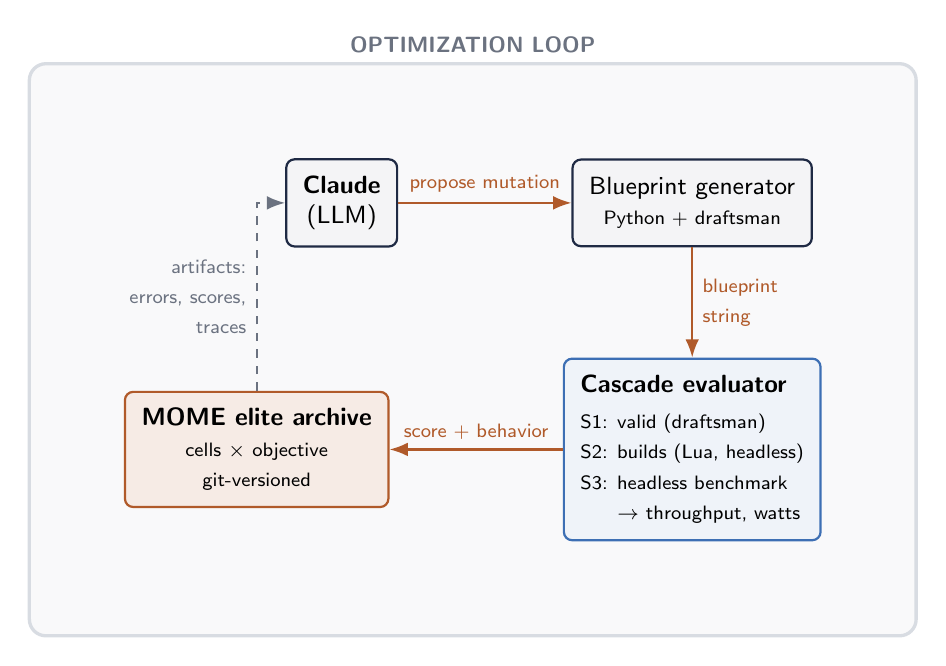
\begin{tikzpicture}[
  font=\small\sffamily,
  node distance=10mm,
  box/.style={draw=forgeNavy,fill=forgeNavy!5,rounded corners=3pt,
              align=center,inner sep=6pt,minimum height=11mm,thick},
  eval/.style={draw=forgeSteel,fill=forgeSteel!8,rounded corners=3pt,
               align=left,inner sep=6pt,thick},
  arc/.style={->,>=Latex,thick,forgeCopper},
  feed/.style={->,>=Latex,thick,forgeAsh,dashed}
]
% nodes
\node[box] (claude) {\textbf{Claude}\\ (LLM)};
\node[box, right=22mm of claude] (gen) {Blueprint generator\\ \scriptsize Python + draftsman};
\node[eval, below=14mm of gen] (casc)
  {\textbf{Cascade evaluator}\\[2pt]
   \scriptsize S1: valid (draftsman)\\
   \scriptsize S2: builds (Lua, headless)\\
   \scriptsize S3: headless benchmark\\
   \scriptsize \hphantom{S3: }$\rightarrow$ throughput, watts};
\node[box, left=22mm of casc, fill=forgeCopper!12, draw=forgeCopper] (arch)
  {\textbf{MOME elite archive}\\ \scriptsize cells $\times$ objective\\ \scriptsize git-versioned};

% arrows
\draw[arc] (claude) -- node[above]{\scriptsize propose mutation} (gen);
\draw[arc] (gen) -- node[right,align=left]{\scriptsize blueprint\\\scriptsize string} (casc);
\draw[arc] (casc) -- node[above,align=center]{\scriptsize score + behavior} (arch);
\draw[feed] (arch.north) |- node[pos=0.25,left,align=right]{\scriptsize artifacts:\\\scriptsize errors, scores,\\\scriptsize traces} (claude.west);

% loop framing
\begin{scope}[on background layer]
  \node[draw=ruleGray, very thick, rounded corners=6pt, fill=forgeAsh!4,
        fit=(claude)(gen)(casc)(arch), inner sep=12mm,
        label={[forgeAsh,font=\footnotesize\sffamily\bfseries]north:OPTIMIZATION LOOP}] {};
\end{scope}
\end{tikzpicture}
\caption[The Factorio Forge optimization loop]{The optimization loop. Claude
proposes a mutation to the blueprint generator; the cascade evaluator culls
invalid candidates cheaply (S1, S2) before paying for a headless benchmark (S3);
surviving elites land in the git-versioned MOME archive, whose artifacts (errors,
scores, traces) feed the next prompt.}
\label{fig:loop}
\end{figure}

\Cref{fig:regimes} shows how the Catalog mediates between the spatial Workshop
regime and the strategic Campaign regime.

\begin{figure}[htbp]
\centering
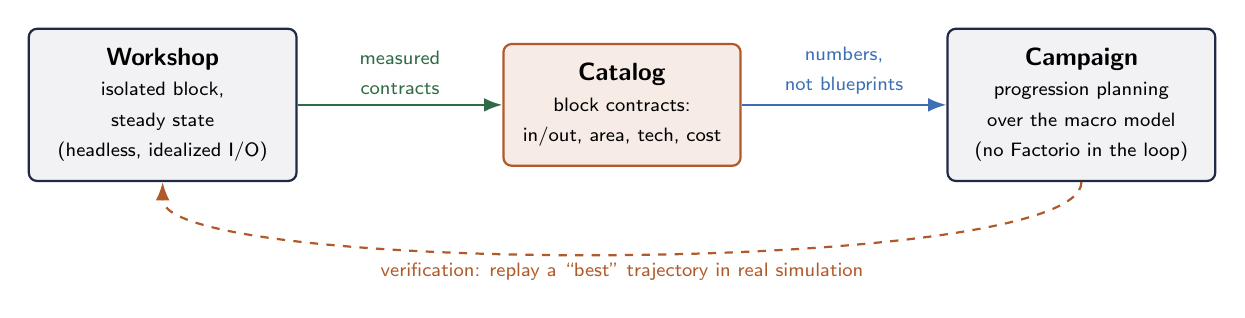
\begin{tikzpicture}[
  font=\small\sffamily,
  reg/.style={draw,rounded corners=3pt,align=center,inner sep=7pt,
              minimum width=34mm,minimum height=14mm,thick},
  cat/.style={draw=forgeCopper,fill=forgeCopper!12,rounded corners=3pt,
              align=center,inner sep=7pt,minimum height=14mm,thick},
  up/.style={->,>=Latex,thick,toolGreen},
  down/.style={->,>=Latex,thick,forgeSteel}
]
\node[reg, draw=forgeNavy, fill=forgeNavy!6] (ws)
  {\textbf{Workshop}\\ \scriptsize isolated block,\\ \scriptsize steady state\\ \scriptsize (headless, idealized I/O)};
\node[cat, right=26mm of ws] (cat)
  {\textbf{Catalog}\\ \scriptsize block contracts:\\ \scriptsize in/out, area, tech, cost};
\node[reg, draw=forgeNavy, fill=forgeNavy!6, right=26mm of cat] (camp)
  {\textbf{Campaign}\\ \scriptsize progression planning\\ \scriptsize over the macro model\\ \scriptsize (no Factorio in the loop)};

\draw[up] (ws.east) -- node[above,align=center,toolGreen]{\scriptsize measured\\ \scriptsize contracts} (cat.west);
\draw[down] (cat.east) -- node[above,align=center,forgeSteel]{\scriptsize numbers,\\ \scriptsize not blueprints} (camp.west);
\draw[down,dashed,forgeCopper] (camp.south) .. controls +(0,-12mm) and +(0,-12mm) ..
  node[below,align=center,forgeCopper]{\scriptsize verification: replay a ``best'' trajectory in real simulation}
  (ws.south);
\end{tikzpicture}
\caption[The three nested regimes and the Catalog interface]{The Catalog as a
surrogate interface. Workshop measures block contracts in headless; the Catalog
stores them as numbers; Campaign plans progressions over those numbers without
running Factorio in the loop. The dashed return arrow is the mandatory
verification step: replay a ``best'' trajectory in real simulation to measure the
prediction-versus-reality gap.}
\label{fig:regimes}
\end{figure}

% =====================================================================
\section{Objectives}
\label{sec:objectives}

The optimization objective is itself a design space. We distinguish
\emph{intrinsic} objectives (measured on the structure) from \emph{extrinsic}
ones (measured against a human reference). The speedrun flips the project from
``exploration with no judge'' to ``there is a record --- beat it.''

\begin{table}[htbp]
\centering
\caption{The eight objective families.}
\label{tab:objectives}
\small
\renewcommand{\arraystretch}{1.2}
\begin{tabularx}{\textwidth}{@{}l X l c@{}}
\toprule
\textbf{Family} & \textbf{Metric} & \textbf{Automatic judge} & \textbf{Feasibility}\\
\midrule
Throughput            & SPM (science/min), items/s & production stats (Workshop) & acquired\\
System efficiency     & \% full lanes, items$\cdot$s$^{-1}\cdot$W$^{-1}$ & measurable in-game & medium\\
Compactness           & throughput/tile, total area & geometry (draftsman) & easy\\
Aesthetics            & symmetry, periodicity, placement entropy & computable on geometry & to define\\
Human portability     & tileability, city-block conformance & structural heuristics & subjective\\
Pedagogy              & coherent start $\rightarrow$ mid $\rightarrow$ endgame books & human + LLM judgment & qualitative\\
Speed (extrinsic)     & time to objective & game timer + leaderboard & costly\\
Robustness            & residual throughput after destroying $k$\% & perturbed simulation & medium\\
\bottomrule
\end{tabularx}
\end{table}

Three remarks shape the objective choice:

\begin{itemize}
\item \textbf{Aesthetics is measurable}, and underexplored. ``Regularity'' and
  ``alignment'' formalize as spatial periodicity (autocorrelation), the fraction
  of grid-aligned entities, and direction entropy. Open question: is an
  aesthetically regular design also performant, or is there a beauty/throughput
  trade-off? --- a perfect MAP-Elites dimension.
\item \textbf{Human portability is in tension with pure optimization.} A
  machine-optimal design is often unreadable dense spaghetti; a portable design
  (city block, reusable beacon book) sacrifices some performance for reusability.
  Optimizing portability means optimizing \emph{for humans} --- probably the most
  concretely useful deliverable, and the terrain that speaks to creators like
  Nilaus.
\item \textbf{Speedrun/TAS has the most solid judge}: an unambiguous metric
  (time), a defined target state, \emph{and} a public human record to beat.
\end{itemize}

The speedrun community already does TAS (Tool-Assisted Speedrun): the
\texttt{AnyPctTAS} mod exists~\cite{anypcttas}, and official leaderboards exist
for both vanilla and Space Age~\cite{speedrun_factorio,speedrun_spaceage}. The
bounds, however, are dated and \textbf{not interchangeable}
(\cref{tab:speedrun}).

\begin{table}[htbp]
\centering
\caption{Speedrun bounds (Any\%) --- dated and non-interchangeable.}
\label{tab:speedrun}
\small
\begin{tabularx}{\textwidth}{@{}l l l X@{}}
\toprule
\textbf{Category} & \textbf{Time} & \textbf{Holder / date} & \textbf{Note}\\
\midrule
Human solo        & ${\sim}$1h27 & Nefrums, vanilla 1.x~\cite{speedrun_nefrums}
  & Solo record has oscillated around 1h21--1h27.\\
Human multiplayer & ${\sim}$1h15 & Team Steelaxe, FFF\#344~\cite{fff344}
  & Vanilla.\\
TAS world record  & 1h21:20 & Gotyoke, 2020, v0.18~\cite{tas_wr_2020}
  & \textbf{Not} a current bound: predates 1.0/2.0, whose mechanics and ratios differ.\\
Space Age TAS     & --- & none exists~\cite{speedrun_spaceage}
  & Virgin territory: a Space Age TAS would be the \emph{first}, not a record beaten.\\
\bottomrule
\end{tabularx}
\end{table}

\begin{toolbox}{AnyPctTAS and the TAS community}
\texttt{AnyPctTAS}~\cite{anypcttas} is a community mod that executes a
pre-authored action sequence to run Factorio start-to-finish without human input
--- effectively the Campaign regime, done by hand, in an action-sequence format.
The existence of a TAS community is doubly useful: it proves the format is
viable, and it provides a human-authored baseline trajectory to compare an
automatically-discovered one against. The absence of a \emph{Space Age} TAS is an
argument \emph{for} the project, not against it.
\end{toolbox}

% =====================================================================
\section{Community diffusion}
\label{sec:diffusion}

Without a community, the collaborative archive stays a solitary exercise.
Diffusion is therefore a project objective, not an afterthought. The first target
is \textbf{Nilaus} (Christian Nilaus), creator of the \emph{Factorio Master
Class} --- the human embodiment of what the machine attempts: take an objective,
invent an optimized method the community adopts.

\paragraph{Exact attribution (critical for credibility).}
Nilaus did \textbf{not} invent the city block. He \textbf{codified and
democratized} it via his Master Class and blueprint books (City Block
$100\times100$, Solar Block, grid-aligned rail
segments)~\cite{nilaus_cityblock,nilaus_masterclass}, to the point of making it
the de~facto standard. The safe and accurate framing is: ``you turned it into a
teachable, standardized method.'' This holds even if the scattered original idea
is not documentable --- and turning an idea into a teachable method is rarer than
having the idea. Telling him ``you invented the city block'' would discredit us in
the first sentence.

His current work --- \emph{True Megabase}, targeting 1M+ SPM in Space Age with
space platforms, asteroid collectors, and quality upcycling~\cite{nilaus_megabase}
--- confirms the initial intuition and makes him a natural target for the
``portability'' and ``Space Age'' objectives.

\paragraph{Pitch angle (positions him as judge-consultant, not subject).}
\begin{quote}\itshape
``You've spent years hand-inventing optimized production methods. The question:
can an automated optimization loop discover methods you wouldn't have found? Not
to replace you --- to give you a \emph{stepping-stone generator}. You set an
objective (a more compact beacon book, a more efficient asteroid ship), it
illuminates the design space and brings you unexpected candidates to refine.''
\end{quote}

\paragraph{Mandatory sequencing.}
Do \emph{not} contact Nilaus before having an artifact that lands. Note the
terrain tension: Phases~0--2 run on vanilla 2.0 single-surface (smelting, green
circuits) --- exactly the most saturated, most hyper-optimized canonical terrain,
where beating a human is hardest. A frontal ``more compact than Nilaus's
standard'' there is a competition lost in advance. So the Wow target must be
\emph{non-comparative}: not ``better than his standard'' but ``a viable design in
a MAP-Elites cell nobody optimizes'' (robustness, aesthetics) --- a ``huh, I
wouldn't have thought of that'' rather than a ``that beats mine.'' Sequence:
demonstrator first (Phase~2-bis, on a terrain of his domain), approach next,
integration as consultant if it sticks.

% =====================================================================
\section{Experiment plan}
\label{sec:plan}

The plan is incremental: each phase yields an exploitable result and de-risks the
next, and each has a measurable success criterion.

\begin{table}[htbp]
\centering
\caption{Experiment phases 0--5.}
\label{tab:phases}
\small
\renewcommand{\arraystretch}{1.25}
\begin{tabularx}{\textwidth}{@{}l L{3.0cm} X@{}}
\toprule
\textbf{Phase} & \textbf{Focus} & \textbf{Success criterion}\\
\midrule
\textbf{0} & Evaluator feasibility &
  An iron-plates/second figure reproducible to $<$1\% from an input blueprint
  string --- materialization (not just reading) must work. Settles Path~A vs
  Path~B. Vanilla 2.0, free.\\
\textbf{1} & Naive single-objective loop &
  The loop converges to \emph{a} stable, reproducible optimum (whether it is the
  canonical is an observation to analyze, not a pass/fail).\\
\textbf{2} & MAP-Elites + archive &
  At least one viable design in a non-canonical cell that we would not have
  designed by hand. Sets up the git-versioned MOME archive.\\
\textbf{2-bis} & Wow demonstrator &
  A design an expert would recognize as ``huh, I wouldn't have thought of that''
  --- non-comparative, on a target creator's terrain. Entry condition for any
  community approach.\\
\textbf{3} & Exotic metrics &
  Switch the lead objective to robustness, energy density, startup latency, or
  measurable aesthetics. Highest real-discovery potential; where stepping stones
  pay off.\\
\textbf{4} & Workshop $\rightarrow$ Campaign &
  Actually play a trajectory judged optimal and measure the
  prediction-versus-reality gap (the central research question). Natural
  objective: minimize time --- converge toward the speedrun/TAS format.\\
\textbf{5} & Space Age (optional) &
  Replay with Space Age entities (foundry, recycler, space platforms, quality).
  The newer terrain is less canonically frozen; producing the \emph{first} Space
  Age TAS lives here.\\
\bottomrule
\end{tabularx}
\end{table}

Phase~0 is the real test and the real risk: it proves the entire ``blueprint
$\rightarrow$ measurement'' chain, whose hardest link is player-less headless
materialization. The toy case is an iron-plate smelting array (infinite ore in,
plates/s out). Everything downstream depends on it working.

% =====================================================================
\section{Limitations}
\label{sec:limits}

We keep these limitations honest and up front; they determine whether the project
succeeds or stalls.

\begin{itemize}
\item \textbf{``Emergence'' is weak-sense.} We claim solutions not anticipated by
  the human optimizer, \emph{not} strong artificial-life emergence. The title and
  ambition stay honest about this.
\item \textbf{Discovered novelty is descriptor-bounded.} MAP-Elites illuminates
  the space \emph{it is told about}, not the space itself. Choosing
  ``area~$\times$~beacons'' will mostly rediscover the compactness/overclock
  trade-off the community already knows. The ``unexpected'' is largely
  pre-determined by the designer of the axes --- the most serious conceptual
  limit.
\item \textbf{The make-or-break link is player-less headless materialization}, not
  statistics reading. Plausible (the \texttt{create\_entity} API exists) but not
  verified by reading code --- the first Phase~0 prototype must establish it.
\item \textbf{Surrogate adversarial exploitation.} The Campaign macro model is not
  merely imprecise; it is gamed by the optimizer (Goodhart) and blind to
  compositional discontinuities (deadlocks). This requires a design countermeasure
  (trust region, out-of-distribution penalty, or top-$k$ re-verification in real
  simulation), not just a-posteriori measurement (see \cref{box:goodhart}).
\item \textbf{MOME archive and semantic git merge are components to build}, not
  free properties. ``One elite per cell'' only holds under the
  (cell~$\times$~objective) keying; a naive text merge corrupts the archive.
\item \textbf{EULA / Factorio ToS.} Headless is free but proprietary (Wube EULA);
  the DLC is account-bound. Thousands of automated runs, multi-instance cloud
  execution, and \emph{a fortiori} publishing results require checking the
  automated-use and multi-instance clauses.
\item \textbf{Speedrun bounds are dated and non-interchangeable.} The TAS WR
  (1h21, 2020) is on Factorio 0.18 vanilla and not comparable to current play;
  there is no Space Age TAS; human Any\% records drift, so any cited figure will
  silently go stale.
\item \textbf{The Space Age DLC is paid} and required for DLC entities, both for
  generation (draftsman after update) and evaluation (headless). Phases~0--3 are
  designed to be feasible on free vanilla 2.0.
\end{itemize}

\begin{notionbox}{Goodhart and adversarial surrogate exploitation}
\label{box:goodhart}
Goodhart's law: ``when a measure becomes a target, it ceases to be a good
measure.'' A surrogate model is a measure; an optimizer that maximizes the
surrogate will steer toward exactly the inputs where the surrogate is
\emph{most wrong in the optimistic direction}. So the error on the
\emph{selected} trajectory is systematically worse than the surrogate's
\emph{average} error --- the optimizer is adversarial against its own model. The
defense is not better averages but structural: a \emph{trust region} (only trust
the surrogate near where it was measured), a novelty/out-of-distribution penalty,
or re-verifying the top-$k$ candidates in real simulation before acting on them.
\end{notionbox}

% =====================================================================
\section{Conclusion}
\label{sec:conclusion}

Factorio Forge takes a well-posed engineering question --- can an automated loop
find factory designs humans would not? --- and equips it with a credible
apparatus: the autoresearch loop for structure~\cite{karpathy_autoresearch}, the
FunSearch~$\rightarrow$~AlphaEvolve lineage for rigor~\cite{alphaevolve_arxiv},
Quality-Diversity for the diversity pressure that defeats canonical
collapse~\cite{qd_reference}, and concrete tooling
(\texttt{factorio-draftsman}~\cite{draftsman_github},
headless benchmarking~\cite{mulark_benchmark}, OpenEvolve~\cite{openevolve}) to
close the loop.

The bet is precise: single-objective search collapses onto the canonical, while
diversity-driven search illuminates an archipelago of unexpected, viable designs,
stored in a multi-objective archive that doubles as a collaborative substrate.
The harder ambition --- the Campaign regime and its surrogate Catalog --- promises
\emph{strategic} emergence (counter-intuitive unlock orders, throwaway
transitional blocks), which may prove more fertile than spatial emergence,
because human players optimize their progression only with coarse heuristics.

We make no inflated claims. The emergence is weak-sense; the novelty is
descriptor-bounded; the make-or-break risk is a concrete piece of Lua plumbing
(player-less materialization), not a grand theory. The incremental plan is built
so that Phase~0 either proves the chain or kills the project early --- which is
exactly the discipline a research project of this kind deserves.

% =====================================================================
\newpage
\bibliographystyle{plainurl}
\addcontentsline{toc}{section}{References}
\bibliography{references}

\end{document}
